\section{Strengthening Theorem \ref{CV} for bounded covering problems} \label{gap}

Theorem \ref{CV} characterizes the integrality gap as the smallest number such that for any point $x\in \dom(P)$, $gx$ dominates a convex combination of points in $S$, i.e. there exists convex combination $\sum_{i=1}^{k}\lambda_ix^i \leq gx$.  In a covering problem, we assume that matrix $A$ in the description of $P$ is a non-negative matrix, hence if $y\geq x$ and $x\in P$ we have $y\in P$. We also assume the right hand side vector in (\ref{P}) is of the form $b\textbf{1}$, i.e. it is a uniform vector. Finally we assume we have bound constraints $x\leq b\textbf{1}$. This class of problems include a broad class of problems. Notice that for a covering problem $\dom(P)=P$.  We show that for these problems, we can make Theorem \ref{CV} stronger in the following sense. 

\tightcuts*

In other words, the integrality gap is the smallest number such that for any $x\in P$, there exists a convex combination $y=\sum_{i=1}^{k}\lambda_ix^i$, such that $A_jy\leq g(A_jx)$ for all $j$ such that $A_jx=b$. 

Notice that the proof of this theorem, same as Theorem \ref{CV}, does not imply a polynomial time algorithm.

Observe that if $C\geq g$, by Theorem \ref{CV}, there is a convex combination of points in $S$ that is dominated by $Cx$, i.e. there exists $\theta\in [0,1]^{k}$, where $\sum_{i=1}^{k}\theta_i=1$, and $x^i\in S$, such that $\sum_{i=1}^{k}\theta_ix^i\leq gx$. The same convex combination also trivially satisfies both requirements in Theorem \ref{tightcuts}. The more interesting direction is the converse. We begin with the following theorem. Suppose $v^1,\ldots,v^r$ are the extreme points of $P$. Assume for each $i=1,\ldots,r$, there exists a convex combination of points in $S$, namely $\sum_{\ell=1}^{k_i} \lambda^i_\ell w^i_\ell$ such that $A_j \sum_{\ell=1}^{k_i} \lambda^i_\ell w^i_\ell \leq CA_jv^i$ for $j$ such that $A_jv^i = b$. Let $z^i = \sum_{\ell=1}^{k_i} \lambda^i_\ell w^i_\ell$.
\begin{lemma}\label{epsilon}
	For any  $i\in\{1,\ldots,r\}$, there exists $\epsilon_i >0$ and ${x^i}\in P$ where ${x^i}\leq \frac{Cv^i-\epsilon_i z^i}{C(1-\epsilon_i)}$.
\end{lemma}
\begin{proof}
	
	Let $u^i(\epsilon) = \frac{Cv^i-\epsilon z^i}{C(1-\epsilon)}$. For $j\in \{1,\ldots,m\}$, let $t_j = A_jz^i-Cb$ and $s_j=A_jv^i-b$. 
	Assume $\epsilon <1$. For $j\in \{1,\ldots,m\}$ such that $A_jz^i\leq Cb$, i.e. $t_j\leq 0$ (this includes $j$ such that $A_jv^i=b$, i.e. $s_j=0$) we have
	\begin{equation*}
	A_j u^i(\epsilon) = \frac{CA_jv^i-\epsilon A_jz^i}{C(1-\epsilon)}\geq \frac{Cb-\epsilon Cb}{C(1-\epsilon)}=b
	\end{equation*}
	Assume $\epsilon \leq C\cdot\min_{j: t_j >0} \frac{s_j}{t_j}$. Notice that $\max_{j: t_j >0} \frac{s_j}{t_j}>0$ since for $j$ such that $t_j>0$, we have $A_jz_i > Cb$ which implies that $A_jv^i>b$, so $s_j>0$. For $j$ such that $t_j>0$ we have
	\begin{align*}
	A_ju^i(\epsilon) &= \frac{CA_jv^i-\epsilon A_jz^i}{C(1-\epsilon)}& \\
	&= \frac{C(b+s_j)-\epsilon (Cb+t_j)}{C(1-\epsilon)}&\\
	&= b+ \frac{Cs_j-\epsilon t_j}{C(1-\epsilon)}&\\
	&\geq b & (\epsilon  \leq C\cdot  \frac{s_j}{t_j}, \mbox{ and } \epsilon <1, \mbox{ so } \frac{Cs_j-\epsilon t_j}{C(1-\epsilon)}\geq 0 )
	\end{align*} 
	Therefore if $\epsilon \leq 1$ and $\epsilon \leq C\cdot\min_{j: t_j >0} \frac{s_j}{t_j}$ we have $Au^i(\epsilon)\geq \textbf{1}b$. Next, we show that we can choose $\epsilon$ so that $ u^i(\epsilon)\geq 0$.
	
	For $\ell\in \{1,\ldots,n\}$, if $z^i_\ell=0$, then we have $u_\ell^i(\epsilon) = \frac{Cv_\ell^i}{C(1-\epsilon)}\geq 0$, since $v^i_\ell\geq 0$ and $\epsilon <1$. Otherwise we have $z^i_\ell>0$. Assume $\epsilon \leq C\cdot \min_{ \ell:z^i_\ell>0}\frac{v^i_\ell}{z^i_\ell}$. Notice that for $\ell$ such that $z^i_\ell>0$, we have $v^i_\ell>0$ since $z^i$ lies in the support of $v^i$ by assumption. This means that $\min_{\ell:z^i_\ell>0}\frac{v^i_\ell}{z^i_\ell}>0$. Now, for $\ell$ such that $z^i_\ell>0$, we have $u^i_\ell(\epsilon) = \frac{Cv_\ell^i-\epsilon z_\ell^i}{C(1-\epsilon)}\geq 0$ by choice of $\epsilon$.
	
	Define $\epsilon_i =\min\{1, C\cdot \min_{j: t_j >0}\frac{s_j}{t_j},C\cdot\min_{\ell: z^i_\ell>0}\frac{v^i_\ell}{z^i_\ell}\}$. By the arguments above $Au^i(\epsilon_i)\geq \textbf{1}b$ and $u^i(\epsilon_i)\geq 0$. Define $x^i$ as follows: For each $j\in \{1,\ldots,m\}$, if $u^i_j(\epsilon_i)\leq b$, then let $x^i_j=u^i_j(\epsilon_i)$, otherwise let $x^i_j=b$. We need to show that $x^i\in P$. Note that clearly $x^i\geq 0$, hence we only need to show that $Ax^i\geq \textbf{1}b$. Suppose for contradiction there is $j\in \{1,\ldots,m\}$ such that $A_jx^i <b$. Since $u^i(\epsilon)\in P$, there must be $\ell^*\in\{1,\ldots,n\}$ such that $u^i_{\ell^*}(\epsilon)>b$, and $A_{j,\ell^*}>0$. But this means that $A_{j,\ell^*}\geq 1$ and $x^i_{\ell^*}=b$. Therefore $A_jx^i \geq  A_{j,\ell^*}x^i_{\ell^*}= A_{j,\ell^*}b\geq b$. \end{proof}
\begin{lemma}\label{tightcutcomb}
	There exists a convex combination of point in $S$ that is dominated by $Cv^i$ for $i=1,\ldots,r$.
\end{lemma}
\begin{proof}
	
	
	We prove something slightly stronger. We show that for $i\in\{1,\ldots,r\}$, and for $j=1,\ldots,i$, the vector $Cv^j$ dominates  a convex combination of $z^1,\ldots,z^i$ and $Cv^{i+1},\ldots,Cv^r$. Note that this is enough to prove our statement since for $i=r$, the statement implies that $Cv^j$ dominates a convex combination of $z^1,\ldots,z^r$ for $j=1,\ldots,r$. 
	
	We proceed by induction on $i$. If $i=1$, we just need to show that $Cv^1$ is dominated by a convex combination of $z^1$ and $Cv^2,\ldots,Cv^r$. By Lemma \ref{epsilon}, there exists $x^1\leq  \frac{Cv^1-\epsilon_1z^1}{C(1-\epsilon_1)}$. We have $x^1\in P$, so we can write $x^1$ as convex combination of $v^1,\ldots, v^r$. We have
	\begin{equation*}
	Cv^1 \geq  \epsilon_1z^1 + C(1-\epsilon_1)x^1 \geq \epsilon_1z^1 + C(1-\epsilon_1) \sum_{\ell=1}^{r}\lambda^1_\ell v^\ell.
	\end{equation*}
	Hence,
	\begin{equation}\label{equation6}
	Cv^1 \geq \frac{\epsilon_1}{1-(1-\epsilon_1)\lambda^1_1}\cdot z^1 + (1-\epsilon_i)\sum_{\ell=2}^{r} \frac{\lambda^1_\ell}{1-(1-\epsilon_1)\lambda_1^1}\cdot Cv^\ell.
	\end{equation}
	Observe that $\frac{\epsilon_1}{1-(1-\epsilon_1)\lambda^1_1}$ and $(1-\epsilon_1)\frac{\lambda^1_\ell}{1-(1-\epsilon_1)\lambda_1^1}$ for $\ell=2,\ldots,r$ form convex multipliers, so the base case holds.
	
	Now consider $i\in \{1,\ldots,r-1\}$. By induction, for $j=1,\ldots,i$ we have
	\begin{equation}\label{IHs}
	Cv^j \geq  \sum_{\ell=1}^{i} \theta^{j}_\ell z^\ell + \sum_{\ell=i+1}^{r}\theta^{j}_{\ell}Cv^\ell.
	\end{equation}
	Suppose we are able to show 
	 \begin{equation}\label{claim} 
	 Cv^{i+1} \geq \sum_{\ell=1}^{i+1} \mu_\ell z^\ell + \sum_{\ell=i+2}^{r}\mu_{\ell}Cv^\ell,\end{equation} 
	where $\mu\geq 0$, and $\sum_{\ell=1}^{r}\mu_{\ell}=1$. Then for $j=1,\ldots,i$ we have
	\begin{align*}
	Cv^j& \geq \sum_{\ell=1}^{i} \theta^{j}_\ell z^\ell +\theta^{j}_{i+1}Cv^{i+1}+  \sum_{\ell=i+2}^{r}\theta^{j}_{\ell}Cv^\ell.& (\mbox{By } \ref{IHs})\\
		& \geq \sum_{\ell=1}^{i} \theta^{j}_\ell z^\ell +\sum_{\ell=1}^{i+1}\theta^{j}_{i+1}\mu_\ell z^\ell+ \sum_{\ell=i+2}^{r}\theta^j_{i+1}\mu_{\ell}Cv^\ell +   \sum_{\ell=i+2}^{r}\theta^{j}_{\ell}Cv^\ell.& (\mbox{By } \ref{claim})\\
		&= \sum_{\ell=1}^{i} (\theta^j_\ell+\mu_{\ell}\theta^j_{i+1}) z^\ell + \mu_{j+1}\theta^j_{i+1}z^{i+1} + \sum_{\ell=i+2}^{r} (\theta^j_\ell+\mu_\ell\theta^j_{i+1})Cv^\ell.&
 			\end{align*} 
		It is easy to see that the multipliers above are convex. Thus, we only need to show the convex combination in (\ref{claim}) exists. This will be similar to what we did in the base case. By Lemma \ref{epsilon}, there exists $\epsilon_{i+1}$ and $x^{i+1}$ such that
		\begin{align*}
		Cv^{i+1}&\geq \epsilon_{i+1}z^{i+1}+ C(1-\epsilon_{i+1})x^{i+1}\\
		&\geq \epsilon_{i+1}z^{i+1}+ (1-\epsilon_{i+1})\sum_{\ell=1}^{k}\lambda_{\ell}Cv^\ell
			\end{align*}
			Applying induction we can replace $Cv^j$ by $ \sum_{\ell=1}^{i} \theta^{j}_\ell z^\ell + \sum_{\ell=i+1}^{r}\theta^{j}_{\ell}Cv^\ell$ for $j=1,\ldots,i$. 
			This means
			\begin{align*}
			(1-(1-\epsilon_{i+1})(\lambda_{i+1}+\sum_{j=1}^{i}\lambda_j\theta^j_{i+1}))Cv^{i+1}&\geq \epsilon_{i+1}z^{i+1}+(1-\epsilon_{i+1})\sum_{j=1}^{i}\lambda_j (\sum_{\ell=1}^{i}\theta^j_\ell z^\ell+ \sum_{\ell=i+2}^{r}\theta^j_\ell Cv^\ell)\\
			&+(1-\epsilon_{i+1})(\sum_{j=1}^{i}\lambda_j \lambda^j_{i+1}+\lambda^i_{i+1})C+ (1-\epsilon_{i+1})\sum_{j=i+2}^{r}\lambda_jCv^{j} 
			\end{align*}
			It is easy to show that  multipliers above are convex.
\end{proof}

\begin{example}

Consider  $\EC(G) = \{x\in [0,2]^E_{\geq 0}: \; x(\delta(U))\geq 2 \mbox{ for $\emptyset \subset U \subset V$}\},$ where $G=(V,E)$ is the graph in Figure \ref{example}. 
\begin{figure}[h]
	\centering
	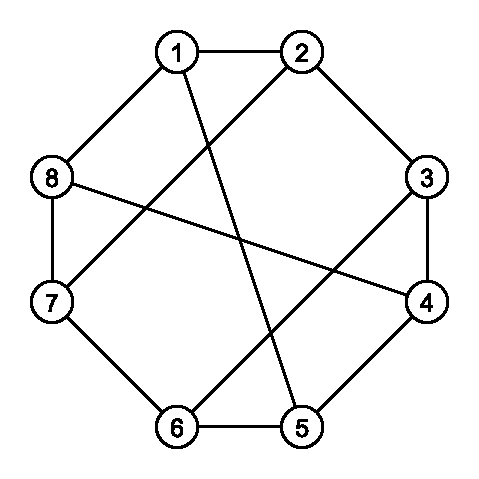
\includegraphics[width=0.2\linewidth]{example.pdf}
	\caption{Graph $G=(V,E)$. Let $H$ be the Hamiltonian cycle of $G$ that contains edges $(1,2),(2,3),(3,4),(4,5),(5,6),(6,7),(7,8),(1,8)$. Let $M= E\setminus H$: $M=\{(1,5),(2,7),(3,6),(4,8)\}$.}
	\label{example}
\end{figure}

Let $v^1$ be the following extreme point of $\EC(G)$: \begin{equation*}
v^1_{e} = \left\{ \begin{array}{ll}
1 & \mbox{if $e\in M$};\\
1/2 & \mbox{if $e\in H$}.
\end{array} \right. 
\end{equation*}
Define $z^1$ to be the following vector:
\begin{equation*}
z^1_{e} = \left\{ \begin{array}{ll}
7/5 & \mbox{if $e= (1,5)$};\\
1 & \mbox{if $e\in M\setminus \{(1,5)\}$};\\
2/5 & \mbox{if $e \in \{(1,8),((4,5))\}$};\\
3/5 & \mbox{if $e\in H\setminus\{(1,8),((4,5))\} $}.
\end{array} \right. 
\end{equation*}
It is easy to check that $z^1$ satisfies the requirement of Theorem \ref{gap} when setting $C=\frac{6}{5}$. In particular, we have $ z^1(\delta(U))\leq \frac{6}{5}v^1(\delta(U))$ for all $\emptyset\subset U \subset V$. Also, is it easy to decompose $z^1$ into a convex combination of integer point in of $\EC(G)$.

Now, we want to set the $\epsilon_i$ in the statement of Lemma \ref{epsilon} to be $2^{-k}$. By Lemma \ref{epsilon}
\begin{equation*}
x^1_{e} = \left\{ \begin{array}{ll}
\frac{2^k-7/6}{2^k-1} & \mbox{if $e= (1,5)$};\\
\frac{2^k-5/6}{2^k-1} & \mbox{if $e\in M\setminus \{(1,5)\}$};\\
\frac{2^k- 2/3}{2\cdot (2^k-1)} & \mbox{if $e \in \{(1,8),((4,5))\}$};\\
\frac{1}{2} & \mbox{if $e\in H\setminus\{(1,8),((4,5))\} $}.
\end{array} \right. 
\end{equation*}
is in $\EC(G)$ for sufficiently large $k$. The vectors defined below $v^2,\ldots,v^7$ are also extreme points of $\EC(G)$.

\begin{table}[h]
	\centering
	\begin{tabular}{ccccccccccccc}
		\toprule
		& (1,5) & (2,7)& (3,6)&(4,8)&(1,2)&(2,3)&(3,4)&(4,5)&(5,6)&(6,7)&(7,8)&(1,8)      \\ \midrule
			$v^2=$ & (0&1&2&1&0&1&1&2&0&0&1&2)  \\
			$v^3=$ & (0&2&2&1&0&0&0&1&1&1&1&2)\\
			$v^4=$ & (1&2&2&2&1&1&1&1&0&0&0&0)\\
			$v^5=$ & (0&2&1&1&1&1&0&1&1&0&0&1)\\
			$v^6=$ & (1&1&1&2&0&1&0&0&1&0&1&1)\\
			$v^7=$ & (1&1&1&2&1&0&1&1&0&1&0&0)\\
				 \bottomrule
	\end{tabular}
\end{table}
Moreover, we have 
\begin{equation*}
x^1 = (1-8\lambda)v^1+ \lambda v^2 + 2\lambda v^3+\lambda v^4+ \lambda v^5+ \lambda v^6 + 2\lambda v^7, \quad \lambda = \frac{1}{24\cdot (2^k-1)}
\end{equation*}
Now, this allows us to rewrite Inequality \ref{equation6} for this example.
\begin{equation*} 
\frac{6}{5}v^1 \geq \frac{3}{4} z^1 +\frac{1}{32}(\frac{6}{5}\cdot v^2) +\frac{1}{16}(\frac{6}{5}\cdot v^3) + \frac{1}{32}(\frac{6}{5}\cdot v^4)+\frac{1}{32}(\frac{6}{5}\cdot v^5) + \frac{1}{32}(\frac{6}{5}\cdot v^6)+ \frac{1}{16}(\frac{6}{5}\cdot v^7).  
\end{equation*}
\end{example}

